%!TEX root = ../OGUSAdoc.tex

The government is not an optimizing agent in \ogindia. The government levies taxes on households, provides transfers to households, levies taxes on firms, spends resources on public goods, and makes rule-based adjustments to stabilize the economy in the long-run. The government can run budget deficits or surpluses in a given year and must, therefore, be able to accumulate debt or savings.

The government sector influences households through two terms in the budget constraint \eqref{EqHHBC}---government transfers $TR_{t}$ and through the total tax liability function $T_{s,t}$, which can be decomposed into the effective tax rate times total income \eqref{EqTaxCalcLiabETR}. In this chapter, we detail the household tax component of government activity $T_{s,t}$ in \ogindia, along with our method of incorporating detailed microsimulation data into a dynamic general equilibrium model.

Incorporating realistic tax and incentive detail into a general equilibrium model is notoriously difficult for two reasons. First, it is impossible in a dynamic general equilibrium model to capture all of the dimensions of heterogeneity on which the real-world tax rate depends. For example, a household's tax liability in reality depends on filing status, number of dependents, many types of income, and some characteristics correlated with age. A good heterogeneous agent DGE model tries to capture the most important dimensions of heterogeneity, and necessarily neglects the other dimensions.

The second difficulty in modeling realistic tax and incentive detail is the need for good microeconomic data on the individuals who make up the economy from which to simulate behavioral responses and corresponding tax liabilities and tax rates.

\ogindia follows the method of \citet{DeBackerEtAl:2017} of generating detailed tax data on effective tax rates and marginal tax rates for a sample of tax filers along with their respective income and demographic characteristics and then using that data to estimate parametric tax functions that can be incorporated into \ogindia.


\section{Effective and Marginal Tax Rates}\label{SecTaxCalcRateTheory}

  Before going into more detail regarding how we handle these two difficulties in \ogindia, we need to define some functions and make some notation. For notational simplicity, we will use the variable $x$ to summarize labor income, and we will use the variable $y$ to summarize capital income.
  \begin{align}
    x_{j,s,t} &\equiv w_{t}e_{j,s}n_{j,s,t} \quad\forall j, t \quad\text{and}\quad E+1\leq s\leq E+S \label{EqTaxCalcLabInc} \\
    y_{j,s,t} &\equiv r_{t}b_{j,s,t} \qquad\:\:\:\,\forall j, t \quad\text{and}\quad E+1\leq s\leq E+S \label{EqTaxCalcLabInc}
  \end{align}

  We can express total tax liability $T_{s,t}$ from the household budget constraint \eqref{EqHHBC} as an effective tax rate multiplied by total income.
  \begin{equation}\label{EqTaxCalcLiabETR}
    T_{s,t} = \tau^{etr}_{s,t}(x_{j,s,t}, y_{j,s,t})\left(x_{j,s,t} + y_{j,s,t}\right)
  \end{equation}
  Rearranging \eqref{EqTaxCalcLiabETR} gives the definition of an effective tax rate ($ETR$) as total tax liability divided by unadjusted gross income, or rather, total tax liability as a percent of unadjusted gross income.

  A marginal tax rate ($MTR$) is defined as the change in total tax liability from a small change income. In \ogindia, we differentiate between the marginal tax rate on labor income ($MTRx$) and the marginal tax rate on labor income ($MTRy$).
  \begin{align}
    \tau^{mtrx} &\equiv \frac{\partial T_{s,t}}{\partial w_t e_{j,s}n_{j,s,t}} = \frac{\partial T_{s,t}}{\partial x_{j,s,t}} \quad\forall j,t \quad\text{and}\quad E+1\leq s\leq E+S \label{EqTaxCalcMTRx} \\
    \tau^{mtry} &\equiv \frac{\partial T_{s,t}}{\partial r_t b_{j,s,t}} = \frac{\partial T_{s,t}}{\partial y_{j,s,t}} \qquad\quad\forall j,t \quad\text{and}\quad E+1\leq s\leq E+S \label{EqTaxCalcMTRy}
  \end{align}
  As we show in Section \ref{SecHHeulers}, the derivative of total tax liability with respect to labor supply $\frac{\partial T_{s,t}}{n_{j,s,t}}$ and the derivative of total tax liability next period with respect to savings $\frac{\partial T_{s+1,t+1}}{b_{j,s+1,t+1}}$ show up in the household Euler equations for labor supply \eqref{EqHHeul_n} and savings \eqref{EqHHeul_b}, respectively. It is valuable to be able to express those marginal tax rates, for which we have no data, as marginal tax rates for which we do have data. The following two expressions show how the marginal tax rates of labor supply can be expressed as the marginal tax rate on labor income times the household-specific wage and how the marginal tax rate of savings can be expressed as the marginal tax rate of capital income times the interest rate.
  \begin{equation}\label{EqMTRx_derive}
    \frac{\partial T_{s,t}}{\partial n_{j,s,t}}  = \frac{\partial T_{s,t}}{\partial w_t e_{j,s}n_{j,s,t}}\frac{\partial w_{t}e_{j,s}n_{j,s,t}}{\partial n_{j,s,t}} = \frac{\partial T_{s,t}}{\partial w_{t}e_{j,s}n_{j,s,t}}w_t e_{j,s} = \tau^{mtrx}_{s,t}w_t e_{j,s}
  \end{equation}
  \begin{equation}\label{EqMTRy_derive}
    \frac{\partial T_{s,t}}{\partial b_{j,s,t}} = \frac{\partial T_{s,t}}{\partial r_{t}b_{j,s,t}}\frac{\partial r_t b_{j,s,t}}{\partial b_{j,s,t}} = \frac{\partial T_{s,t}}{\partial r_t b_{j,s,t}}r_{t} = \tau^{mtry}_{s,t}r_t
  \end{equation}


\section{Microeconomic Data}\label{SecTaxCalcMicro}

  For \ogindia, we use an open source microsimulation model called \taxcalc that uses microeconomic data on U.S. households from the Internal Revenue Service (IRS) Statistics of Income (SOI) Public Use File (PUF).\footnote{\taxcalc is available through an open source repository \href{https://github.com/open-source-economics/Tax-Calculator}{https://github.com/open-source-economics/Tax-Calculator} as well as through a web application \href{https://www.ospc.org/taxbrain/}{https://www.ospc.org/taxbrain/}. Documentation for \taxcalc is available at \href{http://open-source-economics.github.io/Tax-Calculator/}{http://open-source-economics.github.io/Tax-Calculator/} and \href{http://taxcalc.readthedocs.io/en/latest/public_api.html}{http://taxcalc.readthedocs.io/en/latest/public\_api.html}. For users that have not paid for access to the Public Use File (PUF), \taxcalc has an option to use a CPS matched dataset that is publicly available free of charge that has the same general properties as the PUF.}

  \taxcalc starts with the underlying population microeconomic data, in which each observation is a filer with a population weight that renders the sample representative. It then processes the relevant income and demographic characteristics in order to calculate the tax liability of each individual, according to all the rich tax law of the United States tax code. \taxcalc can then calculate effective tax rates for all of these individuals, thereby creating a sample of how ETR's are related to other variables in our \ogindia model, such as total income $x + y$, labor income $x$, and capital income $y$. \taxcalc can also generate marginal tax rates by adding a dollar to each filer's income of a particular type and calculate how the filer's tax liability changes. This is a finite difference calculation of a derivative.

  Figure \ref{FigTaxCalcETRtotinc} shows a scatter plot of $ETR$'s for 43-year-olds in 2017 and unadjusted gross income $x + y$. It is clear that $ETR$ is positively related to income. It is also clear that a significant number of filers have a negative $ETR$. We will discuss in Section \ref{SecTaxCalcFuncs} the functional form \ogindia uses to best capture the main characteristics of these ETR data.

  \begin{figure}[htbp]\captionsetup{width=4.0in}
    \centering
    \caption{\label{FigTaxCalcETRtotinc}\textbf{Plot of estimated $ETR$ functions: $t=2017$ and $s=43$ under current law}}
    \fbox{\resizebox{4.0in}{3.0in}{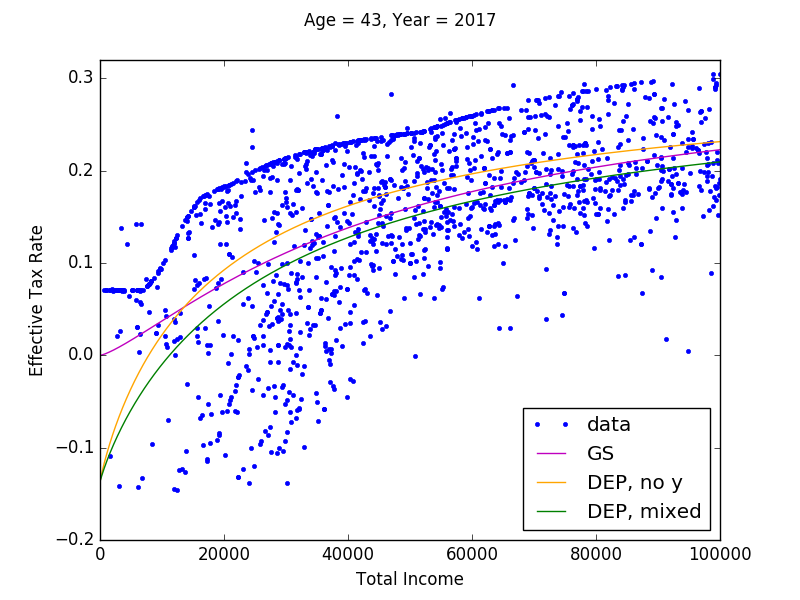
\includegraphics{./images/Compare_ETR_functions.png}}}
  \end{figure}

  Figure \ref{FigTaxCalc3Dtaxrates} shows 3D scatter plots of $ETR$, $MTRx$, and $MTRy$ (and a histogram of the data) with the labor income and capital income, separately, of each age-42 filer in 2017, generated by \taxcalc. This figure presents the main visual evidence for the functional form we use to fit tax functions to these data in Section \ref{SecTaxCalcFuncs}. Figure \ref{FigTaxCalc3Dtaxrates} presents strong evidence that the tax rate---$ETR$, $MTRx$, and $MTRy$---is most accurately modeled as a function of labor income and capital income, separately: $\tau(x,y)$.

  \begin{figure*}[t]\captionsetup{width=6.0in}
    \caption{\label{FigTaxCalc3Dtaxrates}\textbf{Scatter plot of ETR, MTRx, MTRy, and histogram as functions of labor income and capital income from microsimulation model: $t=2017$ and $s=42$ under current law}}
    \fbox{\resizebox{6.0in}{5.0in}{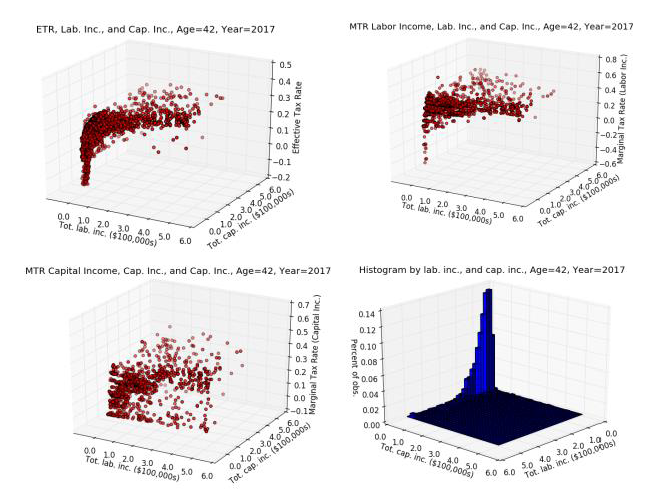
\includegraphics{./images/Age42_2017_scatters.png}}}
    \scriptsize{$^*$Note: Axes in the histogram in the lower-right panel have been switched relative to the other three figures in order to see the distribution more clearly.}
  \end{figure*}


\section{Fitting Tax Functions}\label{SecTaxCalcFuncs}

  In looking at the 2D scatter plot on effective tax rates as a function of total income in Figure \ref{FigTaxCalcETRtotinc} and the 3D scatter plots of $ETR$, $MTRx$, and $MTRy$ in Figure \ref{FigTaxCalc3Dtaxrates}, it is clear that all of these rates exhibit negative exponential or logistic shape. This empirical regularity allows us to make an important and nonrestrictive assumption. We can fit parametric tax rate functions to these data that are constrained to be monotonically increasing in labor income and capital income. This assumption of monotonicity is computationally important as it preserves a convex budget set for each household, which is important for being able to solve many household lifetime problems over a large number of periods.

  \ogindia follows the approach of \citet{DeBackerEtAl:2017} in using the following functional form to estimate tax functions for each age $s=E+1, E+2, ... E+S$ in each time period $t$. Equation \ref{EqTaxCalcTaxFuncForm} is written as a generic tax rate, but we use this same functional form for $ETR$'s, $MTRx$'s, and $MTRy$'s.
  \begin{equation}\label{EqTaxCalcTaxFuncForm}
    \begin{split}
      \tau(x,y) = &\Bigl[\tau(x) + shift_x\Bigr]^\phi\Bigl[\tau(y) + shift_y\Bigr]^{1-\phi} + shift \\
      &\text{where}\quad \tau(x) \equiv (max_x - min_x)\left(\frac{Ax^2 + Bx}{Ax^2 + Bx + 1}\right) + min_x \\
      &\quad\text{and}\quad \tau(y) \equiv (max_y - min_y)\left(\frac{Cy^2 + Dy}{Cy^2 + Dy + 1}\right) + min_y \\
      &\text{where}\quad A,B,C,D,max_x,max_y,shift_x,shift_y > 0 \quad\text{and}\quad\phi\in[0,1] \\
      &\quad\text{and}\quad max_x > min_x \quad\text{and}\quad max_y > min_y
    \end{split}
  \end{equation}
  The parameters values will, in general, differ across the different functions (effective and marginal rate functions) and by age, $s$, and tax year, $t$.  We drop the subscripts for age and year from the above exposition for clarity.

  By assuming each tax function takes the same form, we are breaking the analytical link between the the effective tax rate function and the marginal rate functions.  In particular, one could assume an effective tax rate function and then use the analytical derivative of that to find the marginal tax rate function.  However, we've found it useful to separately estimate the marginal and average rate functions.  One reason is that we want the tax functions to be able to capture policy changes that have differential effects on marginal and average rates.  For example, a change in the standard deduction for tax payers would have a direct effect on their average tax rates.  But it will have secondary effect on marginal rates as well, as some filers will find themselves in different tax brackets after the policy change. These are smaller and second order effects. When tax functions are are fit to the new policy, in this case a lower standard deduction, we want them to be able to represent this differential impact on the marginal and average tax rates. The second reason is related to the first. As the additional flexibility allows us to model specific aspects of tax policy more closely, it also allows us to better fit the parameterized tax functions to the data.

  The key building blocks of the functional form Equation \eqref{EqTaxCalcTaxFuncForm} are the $\tau(x)$ and $\tau(y)$ univariate functions. The ratio of polynomials in the $\tau(x)$ function $\frac{Ax^2 + Bx}{Ax^2 + Bx + 1}$ with positive coefficients $A,B>0$ and positive support for labor income $x>0$ creates a negative-exponential-shaped function that is bounded between 0 and 1, and the curvature is governed by the ratio of quadratic polynomials. The multiplicative scalar term $(max_x-min_x)$ on the ratio of polynomials and the addition of $min_x$ at the end of $\tau(x)$ expands the range of the univariate negative-exponential-shaped function to $\tau(x)\in[min_x, max_x]$. The $\tau(y)$ function is an analogous univariate negative-exponential-shaped function in capital income $y$, such that $\tau(y)\in[min_y,max_y]$.

  The respective $shift_x$ and $shift_y$ parameters in Equation \eqref{EqTaxCalcTaxFuncForm} are analogous to the additive constants in a Stone-Geary utility function. These constants ensure that the two sums $\tau(x) + shift_x$ and $\tau(y) + shift_y$ are both strictly positive. They allow for negative tax rates in the $\tau(\cdot)$ functions despite the requirement that the arguments inside the brackets be strictly positive. The general $shift$ parameter outside of the Cobb-Douglas brackets can then shift the tax rate function so that it can accommodate negative tax rates. The Cobb-Douglas share parameter $\phi\in[0,1]$ controls the shape of the function between the two univariate functions $\tau(x)$ and $\tau(y)$.

  This functional form for tax rates delivers flexible parametric functions that can fit the tax rate data shown in Figure \ref{FigTaxCalc3Dtaxrates} as well as a wide variety of policy reforms. Further, these functional forms are monotonically increasing in both labor income $x$ and capital income $y$. This characteristic of monotonicity in $x$ and $y$ is essential for guaranteeing convex budget sets and thus uniqueness of solutions to the household Euler equations. The assumption of monotonicity does not appear to be a strong one when viewing the the tax rate data shown in Figure \ref{FigTaxCalc3Dtaxrates}. While it does limit the potential tax systems to which one could apply our methodology, tax policies that do not satisfy this assumption would result in non-convex budget sets and thus require non-standard DGE model solutions methods and would not guarantee a unique equilibrium. The 12 parameters of our tax rate functional form from \eqref{EqTaxCalcTaxFuncForm} are summarized in Table \ref{TabTaxCalcTfuncParams}.

  \begin{table}[htbp] \centering \captionsetup{width=5.0in}
  \caption{\label{TabTaxCalcTfuncParams}\textbf{Description of tax rate function $\tau(x,y)$ parameters}}
    \begin{threeparttable}
    \begin{tabular}{>{\footnotesize}c |>{\footnotesize}l }
      \hline\hline
      Symbol & \quad\quad\quad\quad Description  \\
      \hline
      $A$ & Coefficient on squared labor income term $x^2$ in $\tau(x)$ \\
      $B$ & Coefficient on labor income term $x$ in $\tau(x)$ \\
      $C$ & Coefficient on squared capital income term $y^2$ in $\tau(y)$ \\
      $D$ & Coefficient on capital income term $y$ in $\tau(y)$ \\
      $max_x$ & Maximum tax rate on labor income $x$ given $y=0$  \\
      $min_x$ & Minimum tax rate on labor income $x$ given $y=0$ \\
      $max_y$ & Maximum tax rate on capital income $y$ given $x=0$ \\
      $min_y$ & Minimum tax rate on capital income $y$ given $x=0$ \\
      $shift_x$ & shifter $>|min_x|$ ensures that $\tau(x) + shift_x > 0$ despite potentially \\
      & \quad negative values for $\tau(x)$ \\
      $shift_y$ & shifter $>|min_y|$ ensures that $\tau(y) + shift_y > 0$  despite potentially \\
      & \quad negative values for $\tau(y)$ \\
      $shift$ & shifter (can be negative) allows for support of $\tau(x,y)$ to include \\
      & \quad negative tax rates \\
      $\phi$ & Cobb-Douglas share parameter between 0 and 1 \\
      \hline\hline
    \end{tabular}
    % \begin{tablenotes}
    %   \scriptsize{\item[]Note: Maybe put sources here.}
    % \end{tablenotes}
    \end{threeparttable}
  \end{table}

  \begin{figure*}[t]\captionsetup{width=6.0in}
    \caption{\label{FigTaxCalc3DvsPred}\textbf{Estimated tax rate functions of ETR, MTRx, MTRy, and histogram as functions of labor income and capital income from microsimulation model: $t=2017$ and $s=42$ under current law}}
    \fbox{\resizebox{6.0in}{5.0in}{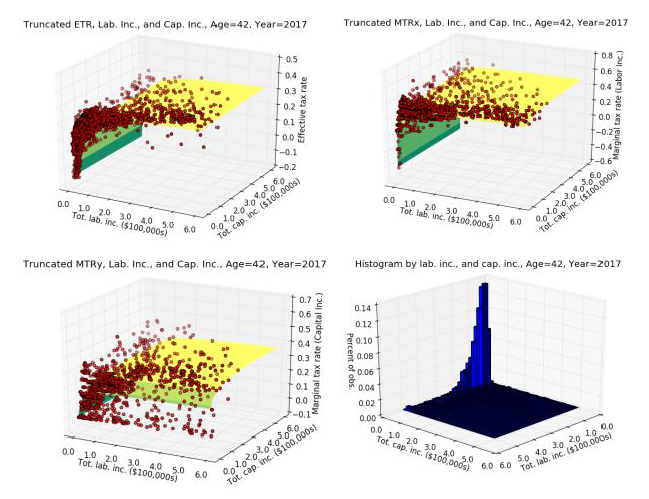
\includegraphics{./images/Age42_2017_vsPred.png}}}
    \scriptsize{$^*$Note: Axes in the histogram in the lower-right panel have been switched relative to the other three figures in order to see the distribution.}
  \end{figure*}

  \begin{table}[htbp] \centering \captionsetup{width=3.0in}
  \caption{\label{TabTaxCalcEst42}\textbf{Estimated baseline current law tax rate function $\tau_{s,t}(x,y)$ parameters for $s=42$, $t=2017$}}
    \begin{threeparttable}
    \begin{tabular}{>{\footnotesize}l |>{\footnotesize}r >{\footnotesize}r >{\footnotesize}r}
    \hline\hline
    Parameter & \multicolumn{1}{c}{\footnotesize{$ETR$}} & \multicolumn{1}{c}{\footnotesize{$MTRx$}} & \multicolumn{1}{c}{\footnotesize{$MTRy$}} \\
    \hline
    $A$ & 6.28E-12 & 3.43E-23 & 4.32E-11 \\
    $B$ & 4.36E-05 & 4.50E-04 & 5.52E-05 \\
    $C$ & 1.04E-23 & 9.81E-12 & 5.62E-12 \\
    $D$ & 7.77E-09 & 5.30E-08 & 3.09E-06 \\
    $max\_{x}$ & 0.80  & 0.71  & 0.44  \\
    $min\_{x}$ & -0.14 & -0.17 & 0.00E+00 \\
    $max\_{y}$ & 0.80  & 0.80  & 0.13 \\
    $min\_{y}$ & -0.15 & -0.42 & 0.00E+00 \\
    $shift\_{x}$ & 0.15  & 0.18  & 4.45E-03 \\
    $shift\_{y}$ & 0.16  & 0.43  & 1.34E-03 \\
    $shift$ & -0.15 & -0.42 & 0.00E+00 \\
    $share$ & 0.84  & 0.96  & 0.86 \\
    \hline
    Obs. (N) & 3,105 & 3,105 & 1,990 \\
    SSE   & 9122.68 & 15041.35 & 7756.54 \\
    \hline\hline
    \end{tabular}
    % \begin{tablenotes}
    %   \scriptsize{\item[]Note: Maybe put sources here.}
    % \end{tablenotes}
    \end{threeparttable}
  \end{table}

  Let $\bm{\theta}_{s,t}=(A,B,C,D,max_x,min_x,max_y,min_y,shift_x,shift_y,shift,\phi)$ be the full vector of 12 parameters of the tax function for a particular type of tax rate, age of filers, and year. We first directly specify $min_x$ as the minimum tax rate and $max_x$ as the maximum tax rate in the data for age-$s$ and period-$t$ individuals for capital income close to 0 ($\$0<y<\$3,000$), and $min_y$ as the minimum tax rate and $max_y$ as the maximum tax rate for labor income close to 0 ($\$0<x<\$3,000$). We then set $shift_x = \min(0,|min_x|)+\ve$ and $shift_y = \min(0,|min_y|)+\ve$ so that the respective arguments in the brackets of \eqref{EqTaxCalcTaxFuncForm} are strictly positive. Then let $shift$ be be the minimum tax rate in the corresponding data minus $\ve$. Let $\bar{\bm{\theta}}_{s,t}=\{min_x,max_x,min_y,max_y,shift_x,shift_y, shift\}$ be the set of parameters we take directly from the data in this way.

  We then estimate five remaining parameters $\tilde{\bm{\theta}}_{s,t}=(A,B,C,D,shift,\phi)$ using the following nonlinear weighted least squares criterion,
  \begin{equation}\label{EqTaxCalcThetaWSSQ}
    \begin{split}
      \bm{\hat{\theta}}_{s,t} = \tilde{\bm{\theta}}_{s,t}:\quad &\min_{\tilde{\bm{\theta}}_{s,t}}\sum_{i=1}^{N} \Bigl[\tau_{i}-\tau_{s,t}\bigl(x_i,y_i|\tilde{\bm{\theta}}_{s,t},\bar{\bm{\theta}}_{s,t}\bigr)\Bigr]^{2} w_i, \\
      &\qquad\text{subject to}\quad A, B, C, D > 0 \quad\text{and}\quad \phi\in[0,1]
    \end{split}
  \end{equation}
  where $\tau_{i}$ is the tax rate for observation $i$ from the microsimulation output, $\tau_{s,t}(x_i,y_i|\tilde{\bm{\theta}}_{s,t},\bar{\bm{\theta}}_{s,t})$ is the predicted tax rate for filing-unit $i$ with $x_{i}$ labor income and $y_{i}$ capital income given parameters $\bm{\theta}_{s,t}$, and $w_{i}$ is the CPS sampling weight of this observation. The number $N$ is the total number of observations from the microsimulation output for age $s$ and year $t$. Figure \ref{FigTaxCalc3DvsPred} shows the typical fit of an estimated tax function $\tau_{s,t}\bigl(x,y|\hat{\bm{\theta}}_{s,t}\bigr)$ to the data. The data in Figure \ref{FigTaxCalc3DvsPred} are the same age $s=42$ and year $t=2017$ as the data Figure \ref{FigTaxCalc3Dtaxrates}.

  The underlying data can limit the number of tax functions that can be estimated. For example, we use the age of the primary filer from the PUF-CPS match to be equivalent to the age of the DGE model household. The DGE model we use allows for individuals up to age 100, however the data contain few primary filers with age above age 80. Because we cannot reliably estimate tax functions for $s>80$, we apply the tax function estimates for 80 year-olds to those with model ages 81 to 100. In the case certain ages below age 80 have too few observations to enable precise estimation of the model parameters, we use a linear interpolation method to find the values for those ages $21\leq s <80$ that cannot be precisely estimated.\footnote{We use two criterion to determine whether the function should be interpolated. First, we require a minimum number of observations of filers of that age and in that tax year. Second, we require that that sum of squared errors meet a predefined threshold.}

  In \ogindia, we estimate the 12-parameter functional form \eqref{EqTaxCalcTaxFuncForm} using weighted nonlinear least squares to fit an effective tax rate function $(\tau^{etr}_{s,t})$, a marginal tax rate of labor income function $(\tau^{mtrx}_{s,t})$, and a marginal tax rate of capital income function $(\tau^{mtry}_{s,t})$ for each age $E+1\leq s\leq E+S$ and each of the first 10 years from the current period.\footnote{We assume that whatever parameters the tax functions have in year 10 persist forever.} That means we have to perform 2,400 estimations of 12 parameters each. Figure \ref{FigTaxCalc3DvsPred} shows the predicted surfaces for $\tau^{etr}_{s=42,t=2017}$, $\tau^{mtrx}_{s=42,t=2017}$, and $\tau^{mtry}_{s=42,t=2017}$ along with the underlying scatter plot data from which those functions were estimated. Table \ref{TabTaxCalcEst42} shows the estimated values of those functional forms.

  The full set of estimated values are calculated in the \href{https://github.com/open-source-economics/OG-USA/blob/master/ogusa/txfunc.py}{\texttt{OG-USA/ogusa/txfunc.py}} module in the \ogindia repository. And the estimated values are stored in the \href{https://github.com/open-source-economics/OG-USA/blob/master/TxFuncEst_baseline.pkl}{\texttt{TxFuncEst\_baseline.pkl}} file.


\section{Factor Transforming Income Units}\label{SecTaxCalcFactor}

  The tax functions $\tau^{etr}_{s,t}$, $\tau^{mtrx}_{s,t}$, and $\tau^{mtry}_{s,t}$ are estimated based on current U.S. tax filer reported incomes in dollars. However, the consumption units of the \ogindia model are not in the same units as the real-world U.S. incomes data. For this reason, we have to transform the income by a $factor$ so that it is in the same units as the income data on which the tax functions were estimated.

  The tax rate functions are each functions of capital income and labor income $\tau(x,y)$. In order to make the tax functions return accurate tax rates associated with the correct levels of income, we multiply the model income $x^m$ and $y^m$ by a $factor$ so that they are in the same units as the real-world U.S. income data $\tau(factor\times x^m, factor\times y^m)$. We define the $factor$ such that average steady-state household total income in the model times the $factor$ equals the U.S. data average total income.
  \begin{equation}\label{EqTaxCalcFactor}
    factor\Biggl[\sum_{s=E+1}^{E+S}\sum_{j=1}^J\lambda_j\bar{\omega}_s\left(\bar{w}e_{j,s}\bar{n}_{j,s} + \bar{r}\bar{b}_{j,s}\right)\Biggr] = \text{Avg. household income in data}
  \end{equation}

  We do not know the steady-state wage, interest rate, household labor supply, and savings \textit{ex ante}. So the income $factor$ is an endogenous variable in the steady-state equilibrium computational solution. We hold the factor constant throughout the nonsteady-state equilibrium solution.


\section{Household Transfers}\label{SecTaxCalcTfers}

  Total transfers to households by the government in a given period $t$ is $TR_t$. The percent of those transfers given to all households of age $s$ and lifetime income group $j$ is $\eta_{j,s}$ such that $\sum_{s=E+1}^{E+S}\sum_{j=1}^J\eta_{j,s,t}=1$. \ogindia currently has the transfer distribution function set to distribute transfers uniformly among the population.
  \begin{equation}\label{EqTaxCalcEtajs}
    \eta_{j,s,t} = \frac{\lambda_j\omega_{s,t}}{\tilde{N}_t} \quad\forall j,t \quad\text{and}\quad E+1\leq s\leq E+S
  \end{equation}
  However, this distribution function $\eta_{j,s,t}$ could also be modified to more accurately reflect the way transfers are distributed in the United States.
